\documentclass[12pt]{article}
\usepackage[T1, T2A]{fontenc}
\usepackage[utf8]{inputenc}
\usepackage[russian]{babel}
\usepackage{hyperref}
\usepackage{graphicx}
\graphicspath{ {../Images/} }

\author{Григорий Матюхин}
\date{\today}
\title{Лабораторная работа \textnumero5.\\Управление системными службами}

\begin{document}
\maketitle
\newpage
\tableofcontents
\newpage
\section{Цель работы}
Получить навыки управления системными службами операционной системы посредством systemd.
\section{Последовательность выполнения работы}

\subsection{Управление сервисами}
\begin{enumerate}
	\item Получите полномочия администратора
	\item Проверьте статус службы Very Secure FTP:
	\item Установите службу Very Secure FTP: \\
	      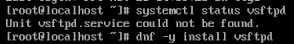
\includegraphics{1.png}
	\item Запустите службу Very Secure FTP:
	\item Проверьте статус службы Very Secure FTP: \\
	      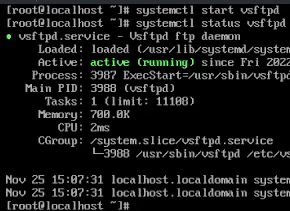
\includegraphics{2.png}
	\item Добавьте службу Very Secure FTP в автозапуск при загрузке операционной системы, используя команду systemctl enable. Затем проверьте статус службы. \\
	      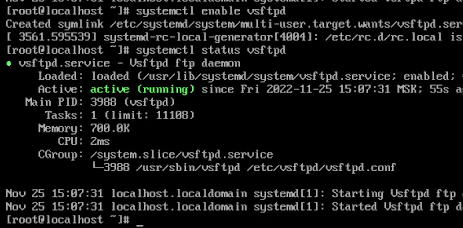
\includegraphics{3.png}
	\item Удалите службу из автозапуска, используя команду systemctl disable, и снова проверьте её статус. \\
	      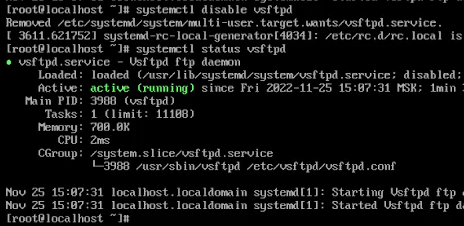
\includegraphics{4.png}
	\item Выведите на экран символические ссылки, ответственные за запуск различных сервисов: \\
	      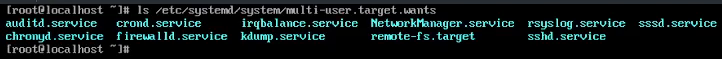
\includegraphics{5.png}
	\item Снова добавьте службу Very Secure FTP в автозапуск и выведите на экран символические ссылки, ответственные за запуск различных сервисов. \\
	      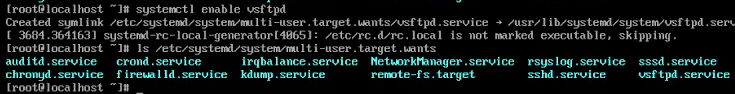
\includegraphics{6.png}
	\item Снова проверьте статус службы Very Secure FTP:
	\item Выведите на экран список зависимостей юнита: \\
	      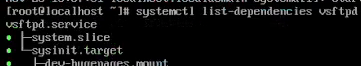
\includegraphics{7.png}
	\item Выведите на экран список юнитов, которые зависят от данного юнита: \\
	      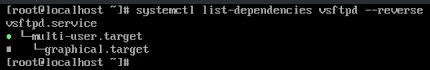
\includegraphics{8.png}
\end{enumerate}

\subsection{Конфликты юнитов}
\begin{enumerate}
	\item Получите полномочия администратора. Установите iptables:
	\item Проверьте статус firewalld и iptables: \\
	      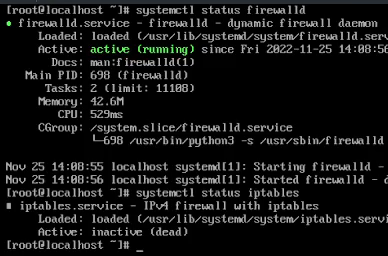
\includegraphics{9.png}
	\item Попробуйте запустить firewalld и iptables: \\
	      
\includegraphics{10.png}
	\item Опишите настройки конфликтов для firewalld при наличии: \\
	      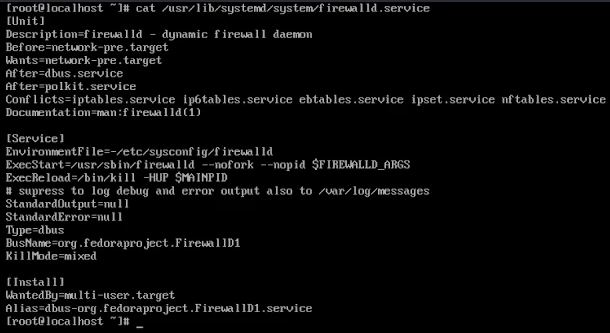
\includegraphics{11.png}
	\item Опишите настройки конфликтов для iptables при наличии: \\
	      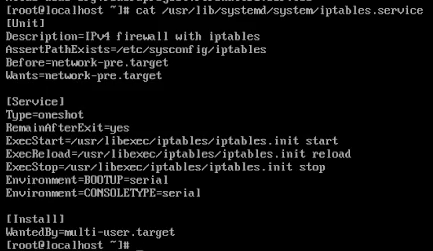
\includegraphics{12.png}
	\item Выгрузите службу iptables и загрузите службу firewalld:
	\item Заблокируйте запуск iptables:
	\item Попробуйте запустить iptables:
	\item Попробуйте добавить iptables в автозапуск: \\
	      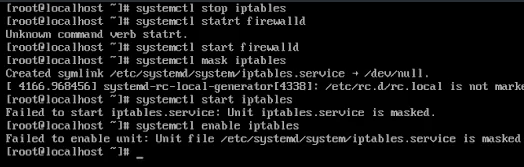
\includegraphics{13.png}
\end{enumerate}

\subsection{Изолируемые цели}
\begin{enumerate}
	\item Получите полномочия администратора. Перейдите в каталог systemd и найдите список всех целей, которые можно изолировать: \\
	      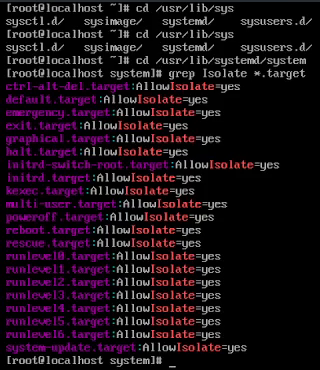
\includegraphics{14.png}
	\item Переключите операционную систему в режим восстановления: \\
	      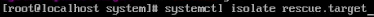
\includegraphics{15.png}
	\item Перезапустите операционную систему: \\
	      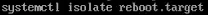
\includegraphics{16.png}
\end{enumerate}

\subsection{Цель по умолчанию}
\begin{enumerate}
	\item Получите полномочия администратора. Выведите на экран цель, установленную по умолчанию: \\
	\item Установаите другую цель как цель по умолчанию: \\
	      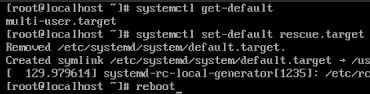
\includegraphics{17.png}
	\item Перегрузите систему командой reboot. Убедитесь, что система загрузилась в установленном режиме:
	\item Верните предыдущую цель как цель по умолчанию: \\
	      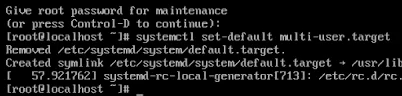
\includegraphics{18.png}
\end{enumerate}

\section{Контрольные вопросы}
\begin{enumerate}
	\item Что такое юнит? Приведите примеры. \\
	      Сущности, которыми управляет \texttt{systemd} и файлы их конфигурации с определённым синтаксисом. Примерами могкт служить сервисы, описывающие фоновые процессы в системе.
	\item Какая команда позволяет вам убедиться, что цель больше не входит в список автоматического запуска при загрузке системы? \\
	      \texttt{systemctl disable <target-name>}
	\item Какую команду вы должны использовать для отображения всех сервисных юнитов, которые в настоящее время загружены? \\
	      \texttt{systemctl list-units --state=loaded}
	\item Как создать потребность (wants) в сервисе?
	      Чтобы цель требовала сервиса, это также можно указать внутри цели с помощью ключа Requires или Wants.
	\item Как переключить текущее состояние на цель восстановления (rescue target)? \\
	      \texttt{systemctl isolate rescue.target}
	\item Поясните причину получения сообщения о том, что цель не может быть изолирована. \\
	      Некоторые юниты не могут быть изолированы, потому что они не имеют ключа \texttt{AllowIsolate=yes} в секции \texttt{[Unit]}
	\item Вы хотите отключить службу systemd, но, прежде чем сделать это, вы хотите узнать, какие другие юниты зависят от этой службы. Какую команду вы бы использовали? \\
	      \texttt{systemctl list-dependencies --reverse service.service}
\end{enumerate}

\section{Вывод}
В ходе выполнения данной работы я получил навыки управления системными службами операционной системы посредством systemd.
\end{document}
